% Für Bindekorrektur als optionales Argument "BCORfaktormitmaßeinheit", dann
% sieht auch Option "twoside" vernünftig aus
% Näheres zu "scrartcl" bzw. "scrreprt" und "scrbook" siehe KOMA-Skript Doku
\documentclass[draft,12pt,a4paper,titlepage,headinclude]{scrartcl}

%%%%%%%%%%%%%%%%%%%%%%%%%%%%%% Formatierung %%%%%%%%%%%%%%%%%%%%%%%%%%%

%keine Einrückung nach leerzeile
\parindent0pt

% Für Kopf und Fußzeilen, siehe auch KOMA-Skript Doku
\usepackage[komastyle]{scrpage2}
\pagestyle{scrheadings}
\setheadsepline{0.5pt}[\color{black}]
\automark[section]{chapter}

%Zitate und Literaturverzeichnis
\usepackage[backend=bibtex,natbib=true,sorting=nyt,style=numeric-comp]{biblatex}
\usepackage[babel]{csquotes}
\bibliography{literatur}

%Zur vernünftigen Dekodierung
\usepackage[T1]{fontenc} %
\usepackage[utf8]{inputenc} %utfx8
\usepackage[german]{babel} %

%Interaktives Dokument
\usepackage[pdfpagelabels=true]{hyperref}%

%Für wissenschaftliches Zitieren
%\usepackage{natbib}

%Schriftarten
%\usepackage{lmodern} %

%Formatierung für Kof- und Fußzeile. Hier gilt entweder ... oder ...!!

%Für eigenen Zeilenabstand
\usepackage{setspace} %

%Für die Seitenformatierung
\usepackage{lscape} %
\usepackage{multicol} %
\usepackage{wallpaper} %

%Styling Inhaltsverzeichnis
\usepackage{tocloft} %

% Zur Formatierung für Kopf und Fußzeilen. Im Allgemeinen ist scrpage2 besser als fancyhdr
\usepackage{scrpage2}
\pagestyle{scrheadings}
\setheadsepline{0.5pt}[\color{black}]

%Einstellungen für Figuren- und Tabellenbeschriftungen
\setkomafont{captionlabel}{\sffamily\bfseries}
\setcapindent{0em} 


%%%%%%%%%%%%%%%%%%%%%%%%%%%%%% Mathematisches %%%%%%%%%%%%%%%%%%%%%%%%%%%

%Pakete für Mathesymbole
\usepackage{latexsym,exscale,stmaryrd} %
\usepackage{amssymb, amsfonts, amstext} %
\usepackage{amsmath, mathtools, amsthm} %

%align nummerierung
\numberwithin{equation}{subsection}

% Weitere Symbole
\usepackage[nointegrals]{wasysym} %
\usepackage{eurosym} %
\usepackage{textcomp} %

%\usepackage{ucs} %

%Für vernünftige Einheiten 
\usepackage[separate-uncertainty, exponent-product = \cdot]{siunitx}
%\usepackage[thinspace,thinqspace,amssymb]{SIunits} %
\usepackage{icomma} %
\usepackage{nicefrac}%

%SI-Einheiten
\usepackage{siunitx}

%%%%%%%%%%%%%%%%%%%%%%%%%%%%%% Grafiken & Tabellen %%%%%%%%%%%%%%%%%%%%%%%%%%%
% Text umfließt Graphiken und Tabellen
% Beispiel:
% \begin{wrapfigure}[Zeilenanzahl]{"l" oder "r"}{breite}
%   \centering
%   \includegraphics[width=...]{grafik}
%   \caption{Beschriftung} 
%   \label{fig:grafik}
% \end{wrapfigure}
% Mehrere Abbildungen nebeneinander
% Beispiel:
% \begin{figure}[htb]
%   \centering
%   \subfigure[Beschriftung 1\label{fig:label1}]
%   {\includegraphics[width=0.49\textwidth]{grafik1}}
%   \hfill
%   \subfigure[Beschriftung 2\label{fig:label2}]
%   {\includegraphics[width=0.49\textwidth]{grafik2}}
%   \caption{Beschriftung allgemein}
%   \label{fig:label-gesamt}
% \end{figure}

%Subfigure nur mit PDF statt Bildern einfügen:
\usepackage{adjustbox}
%\begin{figure}[h]
%  \centering
%  \subfigure[Caption1\label{fig:bild1}]
%  {\begin{adjustbox}{width=0.44\linewidth}\input{bild1}\end{adjustbox}}
%  \hfill
%  \subfigure[Caption2\label{bild2}]
%  {\begin{adjustbox}{width=0.44\linewidth}\input{bild2}\end{adjustbox}}
%  \hfill
%  \subfigure[Caption3\label{bild3}]
%  {\begin{adjustbox}{width=0.44\linewidth}\input{bild3}\end{adjustbox}}
%  \caption{Gesamtcaption}
%  \label{fig:gesamtlabel}
%\end{figure}

%\usepackage{subfigure}




% Caption neben Abbildung
% Beispiel:
% \sidecaptionvpos{figure}{"c" oder "t" oder "b"}
% \begin{SCfigure}[rel. Breite (normalerweise = 1)][hbt]
%   \centering
%   \includegraphics[width=0.5\textwidth]{grafik.png}
%   \caption{Beschreibung}
%   \label{fig:}
% \end{SCfigure}

%Einstellungen für Figuren- und Tabellenbeschriftungen
\setkomafont{captionlabel}{\sffamily\bfseries}
\setcapindent{0em}

%Fuer mehr Platz in den Tabellen
\usepackage{cellspace} %mehr Platz in Tabellen
\addtolength\cellspacetoplimit{3pt}
\newcommand\myhline[1][2pt]{\\[#1]\hline}

%Zum Einbinden von GRafiken
\usepackage{graphicx}% [pdflatex]
\usepackage{xcolor}%

%Für textumflossene Grafiken
\usepackage{wrapfig} %

%Für subfigure
%\usepackage{caption}
\usepackage[font={small}]{caption}
\usepackage{subcaption}

% Caption neben Abbildung
\usepackage{sidecap}

%Für URLs
\usepackage{url}%

%Zum Einbinden von Quelltext
\usepackage{listings-ext} %

%Für chemische Formeln
\usepackage{chemfig} %
\usepackage[version=4]{mhchem} %eingach ueber \ce{} einbinden
%Für chemische Formeln (von www.dante.de)
%% Anpassung an LaTeX(2e) von Bernd Raichle
\makeatletter
\DeclareRobustCommand{\chemical}[1]{%
  {\(\m@th
   \edef\resetfontdimens{\noexpand\)%
       \fontdimen16\textfont2=\the\fontdimen16\textfont2
       \fontdimen17\textfont2=\the\fontdimen17\textfont2\relax}%
   \fontdimen16\textfont2=2.7pt \fontdimen17\textfont2=2.7pt
   \mathrm{#1}%
   \resetfontdimens}}
\makeatother
%erzwinge Fussnote auf selber Seite
\interfootnotelinepenalty=1000

%Zusätzliche Boxen
\usepackage{fancybox}

%\usepackage{framed}
%\usepackage{mathmode}
%\usepackage{empheq}

%Für variable Referenzen
\usepackage{varioref}

%Für Tabellen mit fester Gesamtbreite und variabler Spaltenbreite (im Gegensatz zu tabular)
\usepackage{tabularx}
%\newcommand{\ltab}{\raggedright\arraybackslash} % Tabellenabschnitt linksbündig
%\newcommand{\ctab}{\centering\arraybackslash} % Tabellenabschnitt zentriert
%\newcommand{\rtab}{\raggedleft\arraybackslash} % Tabellenabschnitt rechtsbündig


%Für Gleitobjekte
\usepackage{float} %Für H-Option

\usepackage{multirow} % Zellen von Tabellen zusammenfassen
\usepackage{booktabs} % verschoenert Tabellen
\usepackage{fixltx2e} % Repariert einige Dinge in Bezug auf das setzen von Gleitobjekten http://ctan.org/pkg/fixltx2e
\usepackage{stfloats} % Bei Gleitobjekten (figure,table,...) die ueber zwei Spalten gesetzt werden (Umgebung figure*), funktioniert [tb] http://ctan.org/pkg/stfloats
\usepackage{rotating} % Wird für Text und Grafiken benötigt, die um einen Winkel gedreht werden sollen



%%%%%%%%%%%%%%%%%%%%%%%%%%%%%% Kommandodefinitionen %%%%%%%%%%%%%%%%%%%%%%%%%%%

%Zur Korrektur und Kommentierung
\newcommand{\comment}[1]{\marginpar{\tiny{\textcolor{red}{#1}}}} % ermoeglicht kleine Kommentare am Seitenrand: \comment{Fehler?}
\newcommand{\Comment}[1]{\textcolor{red}{#1}}

%Zur Formatierung in der Matheumgebung
\renewcommand{\t}{\ensuremath{\rm\tiny}} % Tiefgestellter Text in der Matheumgebung wird schoener mit: $\Phi_{\t{Text}}$
\renewcommand{\d}{\ensuremath{\mathrm{d}}} % Die totale Ableitung ist stets aufrecht zu setzen: \d
\newcommand{\diff}[3][]{\ensuremath{\frac{\d^{#1}#2}{\d#3^{#1}}}} % einfache Ableitung nach x: $\ddx{\Phi}$
\newcommand{\pdiff}[3][]{\ensuremath{\frac{\partial^{#1}#2}{\partial#3^{#1}}}} % wie gesprochen, eine partielle Ableitung: \del
\newcommand{\aeqiv}{\ensuremath{\qquad \Longleftrightarrow \qquad}} % Eine Aequivalenz
\newcommand{\folgt}{\ensuremath{\qquad \Longrightarrow \qquad}} % Ein Folgepfeil mit Abstaenden
\newcommand{\corresponds}{\ensuremath{\mathrel{\widehat{=}}}} % Befehl für "Entspricht"-Zeichen
\newcommand{\mi}[1]{\ensuremath{\mathit{#1}}} % italics für griechische Buchstaben in Matheumgebung

%Um nicht so viel schreiben zu müssen...
\newcommand{\bs}[1]{\boldsymbol{#1}}
\newcommand{\ol}[1]{\overline{#1}}
\newcommand{\wtilde}[1]{\widetilde{#1}}
\newcommand{\mrm}[1]{\mathrm{#1}}
\newcommand{\mbf}[1]{\mathbf{#1}}
\newcommand{\mbb}[1]{\mathbb{#1}}
\newcommand{\mcal}[1]{\mathcal{#1}}
\newcommand{\mfrak}[1]{\mathfrak{#1}}

%Abkürzungen
\newcommand{\zB}{z.\,B.\ }
\newcommand{\bzw}{b.\,z.\, w.\ }
\newcommand{\Dh}{d.\,h.\ }
\newcommand{\Gl}{Gl.\ }
\newcommand{\Abb}{Abb.\ }
\newcommand{\Tab}{Tab.\ }

%Farbige Box um eine Formel
%Anwendung:
%\eqbox{
%  \begin{equation}
%    ...
%  \end{equation}
%}
\newcommand{\eqbox}[1]{
  \colorbox{gray!30}{\parbox{\linewidth}{#1}} 
}

%Im Text
\newcommand{\engl}[1]{engl. \textit{#1}}
\newcommand{\zitat}[1]{\footnote{#1}}
\newcommand{\person}[1]{\textsc{#1}}


%Matheoperatoren
\DeclareMathOperator{\tr}{tr}
\DeclareMathOperator{\sgn}{sgn}
\DeclareMathOperator{\diag}{diag}
\DeclareMathOperator{\const}{const}
\DeclareMathOperator{\grad}{grad}
\DeclareMathOperator{\rot}{rot}
\DeclareMathOperator{\divz}{div}


%%%%%%%%%%%%%%%%%%%%%%%%% Quellcode - Formatierung %%%%%%%%%%%%%%%%%%%%%%%%%%%%%%%%%%%%%%

%Um auch Umlaute in den Kommentaren auswerten zu können
\lstset{
literate = {Ö}{{\"O}}1 {Ä}{{\"A}}1 {Ü}{{\"U}}1 {ß}{{\ss}}2 {ü}{{\"u}}1
           {ä}{{\"a}}1 {ö}{{\"o}}1
}

%Formatierung des Quellcode
\lstset{
language=C++,
basicstyle=\footnotesize\ttfamily,
keywordstyle=\bfseries\color{blue},
stringstyle=\color{red},
commentstyle=\itshape\color{green!60!black},
emphstyle = \bfseries\color{red!80!green!60!blue}
%identifierstyle=,
}

%Zum Hervorheben bestimmter Begriffe (z.B. eigene Klassen, etc.)
%\lstset{
%emph = {vector, iterator, std, ostream, istream , ofstream, ifstream, fstream, cmath}
%}

%Nummerirung
\lstset{
numbers=left,
numberstyle=\tiny,
stepnumber=2,
numbersep=5pt,
frame=single,
breaklines=true
framesep=5pt,
numbersep=8pt,
breakindent=3ex
}

%Einbunden über
%\lstinputlisting[caption={blablabla}, language=C++]{name.cpp}

\begin{document}
%Autor, etc.
\newcommand{\versuch}{AG.RBK}
\newcommand{\titel}{Rayleigh Benard Konvektion}
\newcommand{\praktikant}{Michael Lohmann}
\newcommand{\betreuer}{Axel Rosenthal}
\newcommand{\email}{
  \href{mailto:m.lohmann@stud.uni-goettingen.de}
{m.lohmann@stud.uni-goettingen.de} }
\newcommand{\durchfuehrungsdatum}{06.06.2018}
\newcommand{\abgabedatum}{\today}

%Metainformationen
\hypersetup{
      pdfauthor = {\praktikant~ },
      pdftitle  = {\titel: \versuch},
      pdfsubject = {\versuch}
}

\begin{titlepage}
\pagestyle{empty}
\cfoot{}%SeitenNummer wegmachen
\begin{center}
\large{\textbf{Master Forschungspraktikum \\
	  Universit"at G"ottingen, Fakult"at f"ur Physik}} \\
				
%\vspace*{-2cm}
\rule{460pt}{0,01cm}\\[0.5cm]


% ---------------------------------- Titel des Versuches und Institut ----------------------------

\Huge{\textbf{\titel}}\\[0,6cm]

\large{Ausarbeitung zum Versuch \versuch}

%evtl anpassen bei langem Titel
\vspace*{1,0cm}
\end{center}
% --------------------------------------- Betreuer des Versuchs ---------------------------------

\large{
\begin{tabular}{p{80mm}l}
	Name: & \praktikant\\[0,4cm]
	EMail: & \email\\[0,4cm]
	Datum Versuchsdurchf"uhrung: & \durchfuehrungsdatum\\[0,4cm]
	Name Betreuer(in): & \betreuer\\[0,4cm]
	{\scriptsize Kopie der testierten Ausarbeitung erw"unscht:} & {\scriptsize ja} {\tiny{$\square$}} {\scriptsize nein} {\tiny{$\square$}} \\[0,4cm]
	Unterschrift: & 
\end{tabular}
}\\

% --------------------------------------- Rest der Seite nicht ausfuellen -----------------------
%\vspace*{1cm}
\begin{center}
\Large{\textbf{Abgabe}}\\[1.0cm]
\end{center}
\begin{tabular}{p{80mm}l}
Datum: &  Unterschrift Betreuer(in): 
\end{tabular}\\

%\vspace*{1cm}
\begin{center}
\Large{\textbf{Testat}}\\[1.0cm]
\end{center}
\begin{tabular}{p{80mm}l}
Datum:  & Name Pr"ufer(in):\\[0,4cm]
Punktezahl: & Unterschrift: \\[0,4cm]
Note:& 
\end{tabular}
\end{titlepage}

\cleardoublepage
\tableofcontents
\thispagestyle{empty}
\cleardoublepage

\setcounter{footnote}{0}
\setcounter{page}{1}

\pagenumbering{arabic}

\newpage

\section{Motivation}
\label{sec:einleitung}

Konvektion ist ein Phänomen in Strömungen, welches an den unterschiedlichsten Orten auftritt.
Es beschreibt den Transport von Energie mittels eines Teilchenstroms und findet sich zum Beispiel in Erdkern und -mantel, in der Athmosphäre, aber auch in Meeresströmungen und der Kaffeetasse.

Die \textsc{Rayleigh-Bérnard}-Konvektion ist ein Spezialfall, wobei der Energiegradient durch eine heiße Unterseite und eine kalte Oberseite eines mit einem Fluid gefüllten Gefäßes hervorgerufen wird.
Die höhere Temperatur an der Unterseite sorgt dafür, dass sich das Fluid erwärmt, wobei es eine geringere Dichte bekommt.
Durch Auftriebskräfte strebt die Flüssigkeit nun nach oben, bis sie an der oberen Platte angekommen ist und sich dort abkühlt.
Dabei sinkt erneut die Dichte und sie sinkt wieder nach unten.

Als Beispiel lässt sich hier die Mantelkonvektion im Inneren der Erde anbringen, da der äußere Erdkern durch radioaktiven Zerfall thermisch auf über $3000^\circ$ erwärmt wird und die Erdkruste durch Abstrahlung deutlich kühler ist.
Aber auch in der Athmosphäre wird der Boden durch Sonneneinstrahlung erwärmt und die Stratosphäre bildet den oberen Rand.

Auch in der Industrie ist es ein wichtiges Phänomen, welches zum Beispiel bei dem Betrieb eines Hochofens beachtet werden muss \cite{hochofen}.


Viele der genannten Systeme sind kugelsymmetrisch, das hier vorgestellte Experiment wurde jedoch in einem Kubus durchgeführt.
Es bilden sich jedoch trotzdem ähnliche Strömungsmuster, wie sich herrausstellt.


\newpage
\section{Modell und Beschreibung}
\label{sec:theorie}

\subsection{Bewegungsgleichung}
Die Rayleigh-Bénard-Konvektion (RBK) wird durch die \textsc{Navier-Stokes}-Gleichung
\begin{align}
	\frac{\partial \vec{v}}{\partial t} + \left(\vec{v}\cdot\nabla\right)\vec{v} &= 
	-\frac{1}{\rho_0}\nabla p+\nu\nabla^2\vec{v}-\vec{g}\alpha\Delta T\quad,\label{eq:nast}
\end{align}
die Kontinuitätsgleichung
\begin{align}
	\nabla\cdot\vec{v} &= 0\label{eq:konti}
\end{align}
und Temperatur-Transport-Gleichung  
\begin{align}
	\frac{\partial T}{\partial t} + \left( \vec{v}\cdot\nabla \right)\vec{v} = \kappa\nabla^2T\label{eq:tempera}
\end{align}
beschrieben.
Hierbei sind $\vec{v}$ das dreidimensionale Geschwindigkeitsfeld, $p$ das Druckfeld und $T$ das Temperaturfeld.
Die Konstante $\alpha$ der Ausdehnungskoeffizient, $\vec{g}=g\hat{e}_z$ die Erdbeschleunigung (in dem gewählten Bezugssystem in $z$-Richtung), $\Delta T$ die Temperaturdifferenz der Randbedingungen, $\nu$ die dynamische Viskosität und $\kappa$ die thermische Leitfähigkeit.
Die für die Lösung des Gleichungssystemes benötigen Randbedingungen der Geschwindigkeit sind feste Ränder, bzw. $\vec{v}=0$ am Rand.
Die Temperatur am unteren und oberen Rand bei $z=0,L$ ist durch Heiz- bzw. Kühlelemente bestimmt ($L$ bezeichnet die Höhe der Zelle).
Am unteren Rand liegt die Temperatur $T(z=0)=T_0$ und am oberen die Temperatur $T(z=L)=T_0-\Delta T$ an.
Um RBK zu erhalten muss $\Delta T\geq0$ gelten.

Bei dem Aufstellen der Gleichungen wurde von einem inkompressiblen Fluid ausgegangen.
Allerdings wird für den Auftriebsterm in der Navier-Stokes-Gleichung \eqref{eq:nast} angenommen, dass sich die Dichte leicht mit der Temperatur variiert und somit eine lineare
\begin{align*}
	\rho=\rho_0\left( 1 - \alpha\left( T - T_0 \right) \right)
\end{align*}
Abhängigkeit besteht.
Diese Näherung ist auch als \textsc{Boussinesq}-Näherung bekannt.

Zur besseren Vergleichbarkeit von verschiedenen Experimenten wird eine Entdimensionalisierung durchgeführt.
Dazu werden alle vorkommenden Konstanten und Variablen in Abhängigkeit von charakteristischen Größen des Versuchs ausgedrückt.
Z.B. Ortsvektoren in Einheiten der Höhe $\vec{r}=\vec{r'} L$, Zeiten in Einheiten der Höhe und Viskosität $t=t' \frac{L^2}{\nu}$ und Geschwindigkeiten in Einheiten des Orts und der Zeit $\vec{v}=\vec{v'}\frac{\nu}{L}$.
Die mit $'$ versehenen Variablen sind die jeweiligen dimensionslosen Variablen, bei welchen im Folgenden zur besseren Lesbarkeit die $'$ weggelassen werden.

Somit lässt sich die Navier-Stokes-Gleichung auch zu
\begin{align}
	\frac{\partial \vec{v}}{\partial t}+\left( \vec{v}\cdot\nabla \right)\vec{v} &= -\nabla p + Pr\nabla^2\vec{v}+PrRaT\hat{e}_z
\end{align}
umformen, wobei der Druck hier nur die Rolle eines Potentiales hat, das die Divergenzfreiheit gewährleistet.
Die anderen Gleichungen haben jeweils die gleiche Form.
Zu erkennen ist, dass es zwei dimensionslose Parameter gibt:
Die Prandtl-Zahl
\begin{align}
	Pr=\frac{\nu}{\kappa}\label{eq:Pr}
\end{align}
welche das Verhältnis von viskoser zu thermischer Diffusion beschreibt.
Sie hängt offensichtlich nur von Fluid- und nicht von Experiment-Eigenschaften ab.
Die zweite ist die Rayleigh-Zahl
\begin{align}
	Ra=\frac{g\alpha\Delta T L^3}{\kappa\nu}.\label{eq:Ra}
\end{align}
welche das Verhältnis von thermischem Ausgleich durch Auftrieb zu dem durch thermische Diffusion ist.
Es gibt einen kritischen Wert $Ra_\text{crit}$ ab dem der thermische Ausgleich von reiner Diffusion zu einer zusätzlichen advektiven Bewegung wechselt.

In Tabelle \ref{tab:par} im Anhang sind Kennzahlen für verschiedene Systeme und die jeweiligen Stoffparameter aufgeführt.
%Beschreibung der Rayleigh Zahl in der Zelle

\subsection{Nusselt-Zahl}
Zur Beschreibung des Wärmetransportes wird die Nusselt-Zahl
\begin{align*}
	Nu=\frac{\text{gesamter Wärmetransport}}{\text{rein diffusiver Wärme Transport}}
\end{align*}
verwendet.
Diese ergibt unterhalb der kritischen Rayleigh-Zahl $Nu=1$, aufgrund von rein diffusiven Transports.
Oberhalb dieser ergibt sich eine Zahl $Nu>1$, zunehmend mehr Wärme transportiert wird.
Aufgrund der Randbedingung der Geschwindigkeit gibt es am Rand keine Advektion.
Es muss sich also eine diffusive Randschicht ausbilden.
Ist die Advektion im inneren der Zelle groß genug, wird keine Wärme mehr diffusiv übertragen und somit muss die thermische Randschicht einen steilen Gradienten der Temperatur aufweisen, für welchen die Nussel-Zahl gegeben ist durch
\begin{align}
	Nu=\frac{L}{2\delta}.
\end{align}
Das $\delta$ ist die Dicke der thermischen Randschicht.
Eine weitergehende Beschreibung der Nusselt-Zahl und möglicher Abhängigkeiten zu den anderen Parameters kann im Buch von J.S. Turner \cite{Bef} in den Kapiteln 7.1.1, 7.1.3 und 7.3.1 nachgelesen werden.
%Bild des Temperaturprofils aus der Simulation

\subsection{Bewegungsformen und Profile}
Auf ungemittelten Zeitskalen zeigen sich auch Strömungsformen, wie z.B. Plumes.
Plumes sind o.B.d.A. aufsteigende Strömungen, die von einer Auftriebsquelle ausgehen, welche häufig als Punktquelle genähert wird.
Sie sind ähnlich zu einem Jet, allerdings durch Dichteunterschiede getrieben.
Ihren Namen erhielten diese Strömungen aufgrund ihrer Form, den während der Aufströmung dehnen sie sich aus und bilden einen Pilzartigen Kopf.
Eine solche Strömung kann z.B. an einer Rauchfahne beobachtet werden, die sich von einerm Feuer ausbildet.
Außerdem sind Mantelplumes, als Plumes im Erdmantel, eine Quelle für Vulkanische Aktivität.
Ein Schema für einen solchen Plume ist in der Abbildung \ref{fig:plume} zu sehen.
\begin{figure}[!ht]
\centering
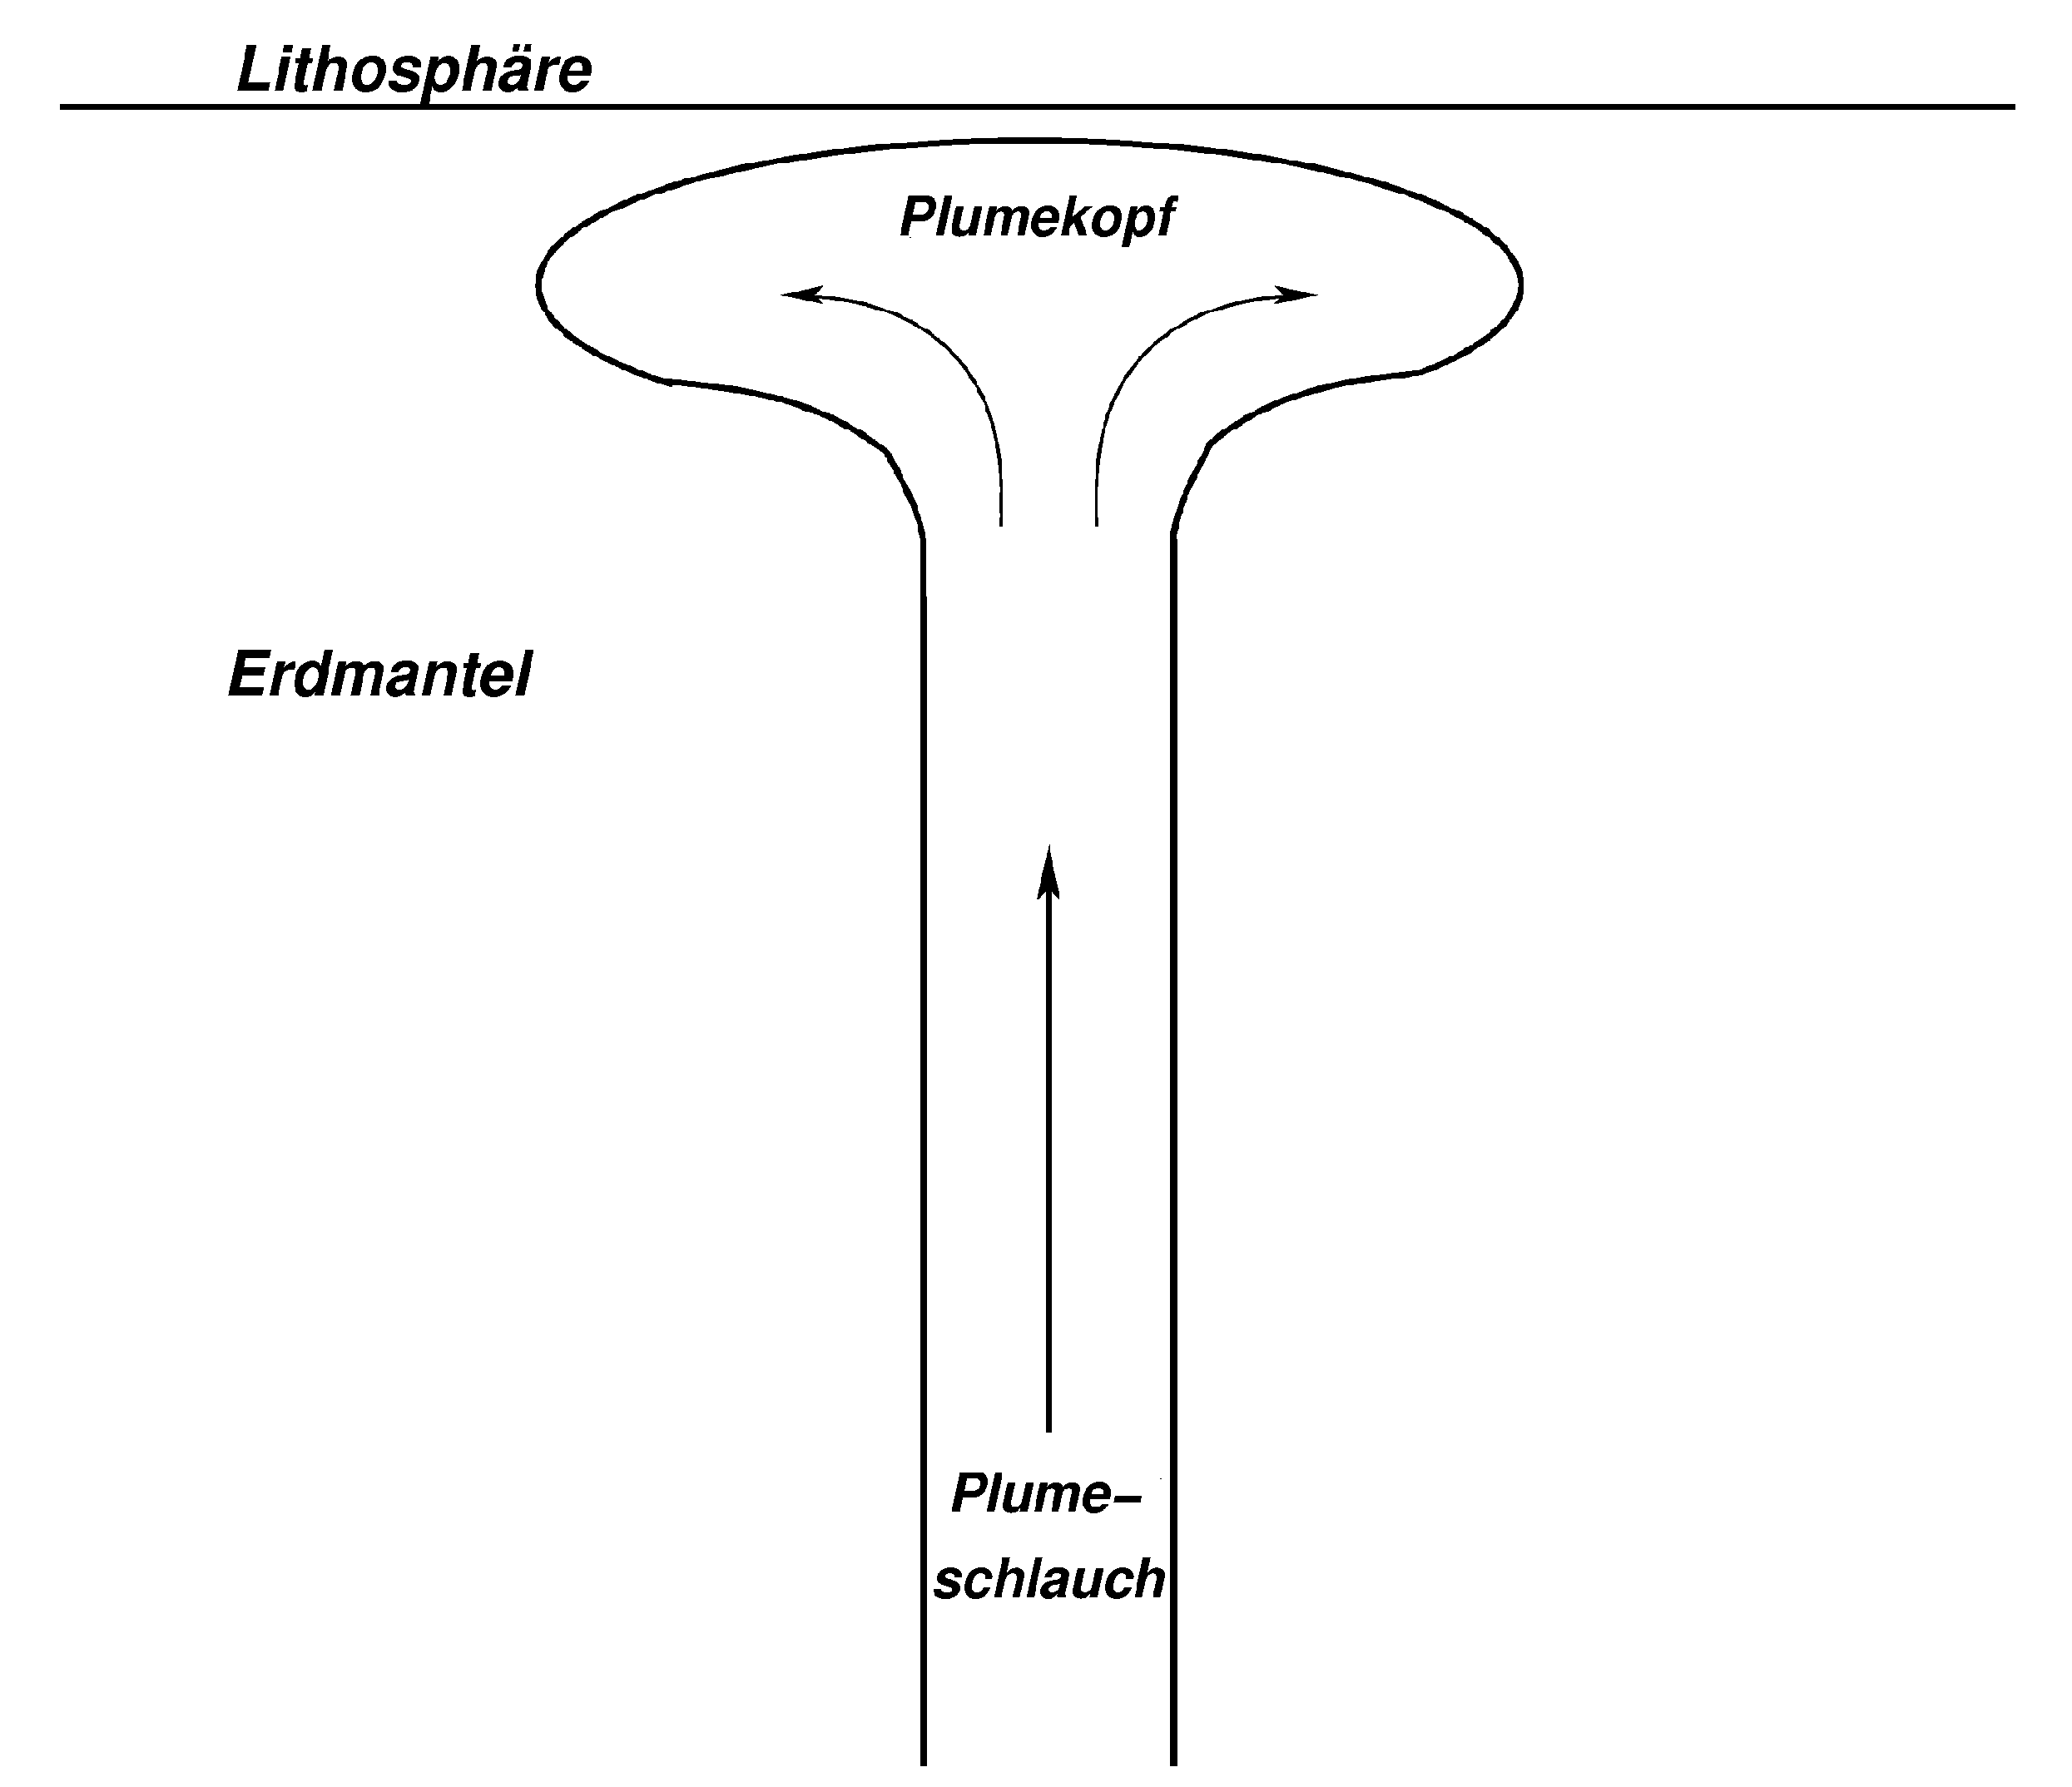
\includegraphics[width=0.5\textwidth]{Plume.png}
\caption{Schema eines Mantelplumes.\protect\footnotemark Der untere Teil des Plumes stellt eine Auftriebsgetriebene Aufströmung dar, welche oben an der Grenze des Mantels einen Pilzkopfartige Form annimmt. An dem Ort des Auftreffens steigt die Warscheinlichkeit vukanischer Aktivität.}
\label{fig:plume}
\end{figure}
\footnotetext{\url{https://de.wikipedia.org/w/index.php?title=Plume_\%28Geologie\%29\&oldid=168415045} vom 02.03.2018 13:30}
Eine sehr detallierte Analyse von Plumes ist im Buch von J.S. Turner \cite{Bef} im Kapitel 6 zu finden.\\

Diese treiben die LSC (Large Scale Circulation) an.
Diese können von hexagonalen Zellen zu Walzen förmigen Strukturen und anderen reichen.
Um diese Formen auch im sehr Turbulenten Strömungen zu erkennen muss das Geschwindigkeitsfeld zeitlich gemittelt werden. 
Bei kleinen Rayleigh-Zahlen ist der Turbulenzgrat noch gering, so dass das zeitliche Mittel nur kurz durchgeführt werden muss um diese Strukturen zu sehen.\\
\begin{figure}[!ht]
\centering
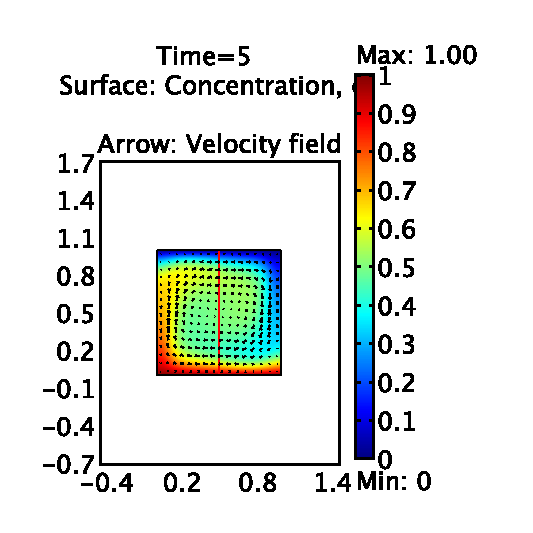
\includegraphics{1e5.eps}
\caption{Ergenis einer Simulation für $Ra=10^5$.}
\label{fig:1e5_num}
\end{figure}

Wie häufig ein solcher Plume ensteht und wie stark er eine LSC antreibt hängt von der Rayleigh-Zahl ab und spiegelt sich im Turbulenzgrad wieder.
An dieser Stelle lohnt es nicht hier weiter ins Detail zu gehen, da dies eine längere Diskussion ist, der Leser ist wieder auf das Buch von J.S. Tuner \cite{Bef} Kapitel 7.3 verwiesen.
Diese Plumes sind gut zu messen, da sie eine deutlich unterschiedliche Temperatur und Dichte zur Umgebung haben.
Hierauf wird in den Kapiteln \ref{sec:schatte} und \ref{sec:profile} näher eingegangen.

\newpage
\section{Experiment und Setup}
\label{sec:durchfuehrung}

Die RBK wird in einer kubischen Plexiglas Zelle mit $20\si{\centi\meter}$ simuliert.
Diese wird von oben und unten mithilfe einer Metallplatte geheizt und gekühlt entsprechen der Randbedingung.
Innerhalb der Zelle befinden sich Thermistoren, welche unten genauer erläutert werden um die Temperatur zu messen.
Es gibt eine Phalanx an Thermistoren in festen Abständen und einen frei in $z$-Richtung verfahrbaren.
Erstere dienen zur zeitlichen Korrelation auf, oder absteigender Strukturen, wie z.B. Plumes.
Letzter wird zur Messung der mittleren Temperatur an bestimmten orten verwendet.
Ebenfalls sind Thermistoren zu Messung der Plattentemperaturen vorhanden.

Die Widerstände der Thermistoren werden entweder durch ein Multimeter oder durch eine Wheatstonebrücke bestimmt, welche ebenfalls weiter unten beschrieben wird.

\subsection{Thermistoren}
Ein Thermistor ist ein Temperaturabhängiger Widerstand.
Diese Abhängigkeit muss vorher bestimmt werden um aus den Widerständen Temperaturen zu errechnen.
Die hier verwendeten Thermistoren sind sogenannte Heißleiter, also Widerstände bei denen der Widerstand bei steigenden Temperaturen fällt (NTC-Widerstände).

\subsection{Wheatstonebrücke}
Eine Wheatstonebrücke ist eine Schaltung, bei der durch mehrere Widerstände und der Messung einer Spannung ein Widerstand bestimmt werden kann.
Eine repräsentative Schaltung kann in der Abbildung \ref{fig:wheat} eingesehen werden.
\begin{figure}[!ht]
\centering
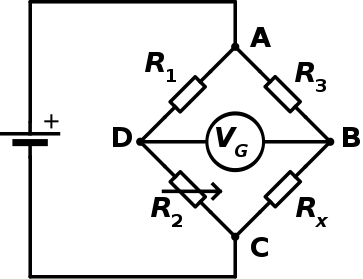
\includegraphics[width=0.5\textwidth]{Wheatstone.png}
\caption{Schaltung einer Wheatstonebrücke.\protect\footnotemark}
\label{fig:wheat}
\end{figure}
\footnotetext{\url{https://en.wikipedia.org/w/index.php?title=Wheatstone_bridge&oldid=819699391} vom 01.02.2018 11:34}

Die Widerstände $R_1$ und $R_3$ sind bekannt.
Das Potentiometer $R_2$ wird zur Eichung der Brücke verwendet und der unbekannte Widerstand $R_x=R_{th}$ ist der Thermistor.
Ist die Brücke abgeglichen, sprich die Spannung $V_G=0$, so gilt für die Widerstände
\begin{align*}
	\frac{R_3}{R_1}=\frac{R_{th}}{R_2}. %das ist glaube ich Falsch
\end{align*}
%weiter beschreiben

%Niquist Shannen Theorem erklären

\subsection{Spektrum einer Zeitserie und Korellation}
%erklären


\newpage
\section{Ergebnisse}
\label{sec:auswertung}

\subsection{Schattenprojektion}
\label{sec:schatte}
Mithilfe einer Schattenprojektion kann Bewegung im Fluid sichtbar gemacht werden.
Zu erkennen sind Dichte unterschiede, welche insbesondere and rapide auf- und absteigenden Plumes zu erkennen ist, da dort die unterschiede größer sind.
Um die Geschwindigkeit der Plumes zu bestimmen wird deren Bewegung auf einem Schirm beobachtet und die laufzeit zwischen vorher festgelegten punkten gemessen.
Die lauflänge auf den Schirm muss noch mithilfe des Strahlensatzes umgerechnet werden um die korrekte Strecke zu erhalten.\\
Um die Position der Plumes in der Zelle genauer einschränken zu können wird orthogonal zur ersten Richtung erneut gemessen.
Mit dieser Methode lässt sich einschränken in welchem Quadranten die Plumes auf und absteigen.
%Skizze der von uns gemessenen quadranten
\\
%Tabelle der Daten mit Fehlern und Raynolds Zahl



\subsection{Störfrequenzen}

\begin{figure}[!ht]
\centering
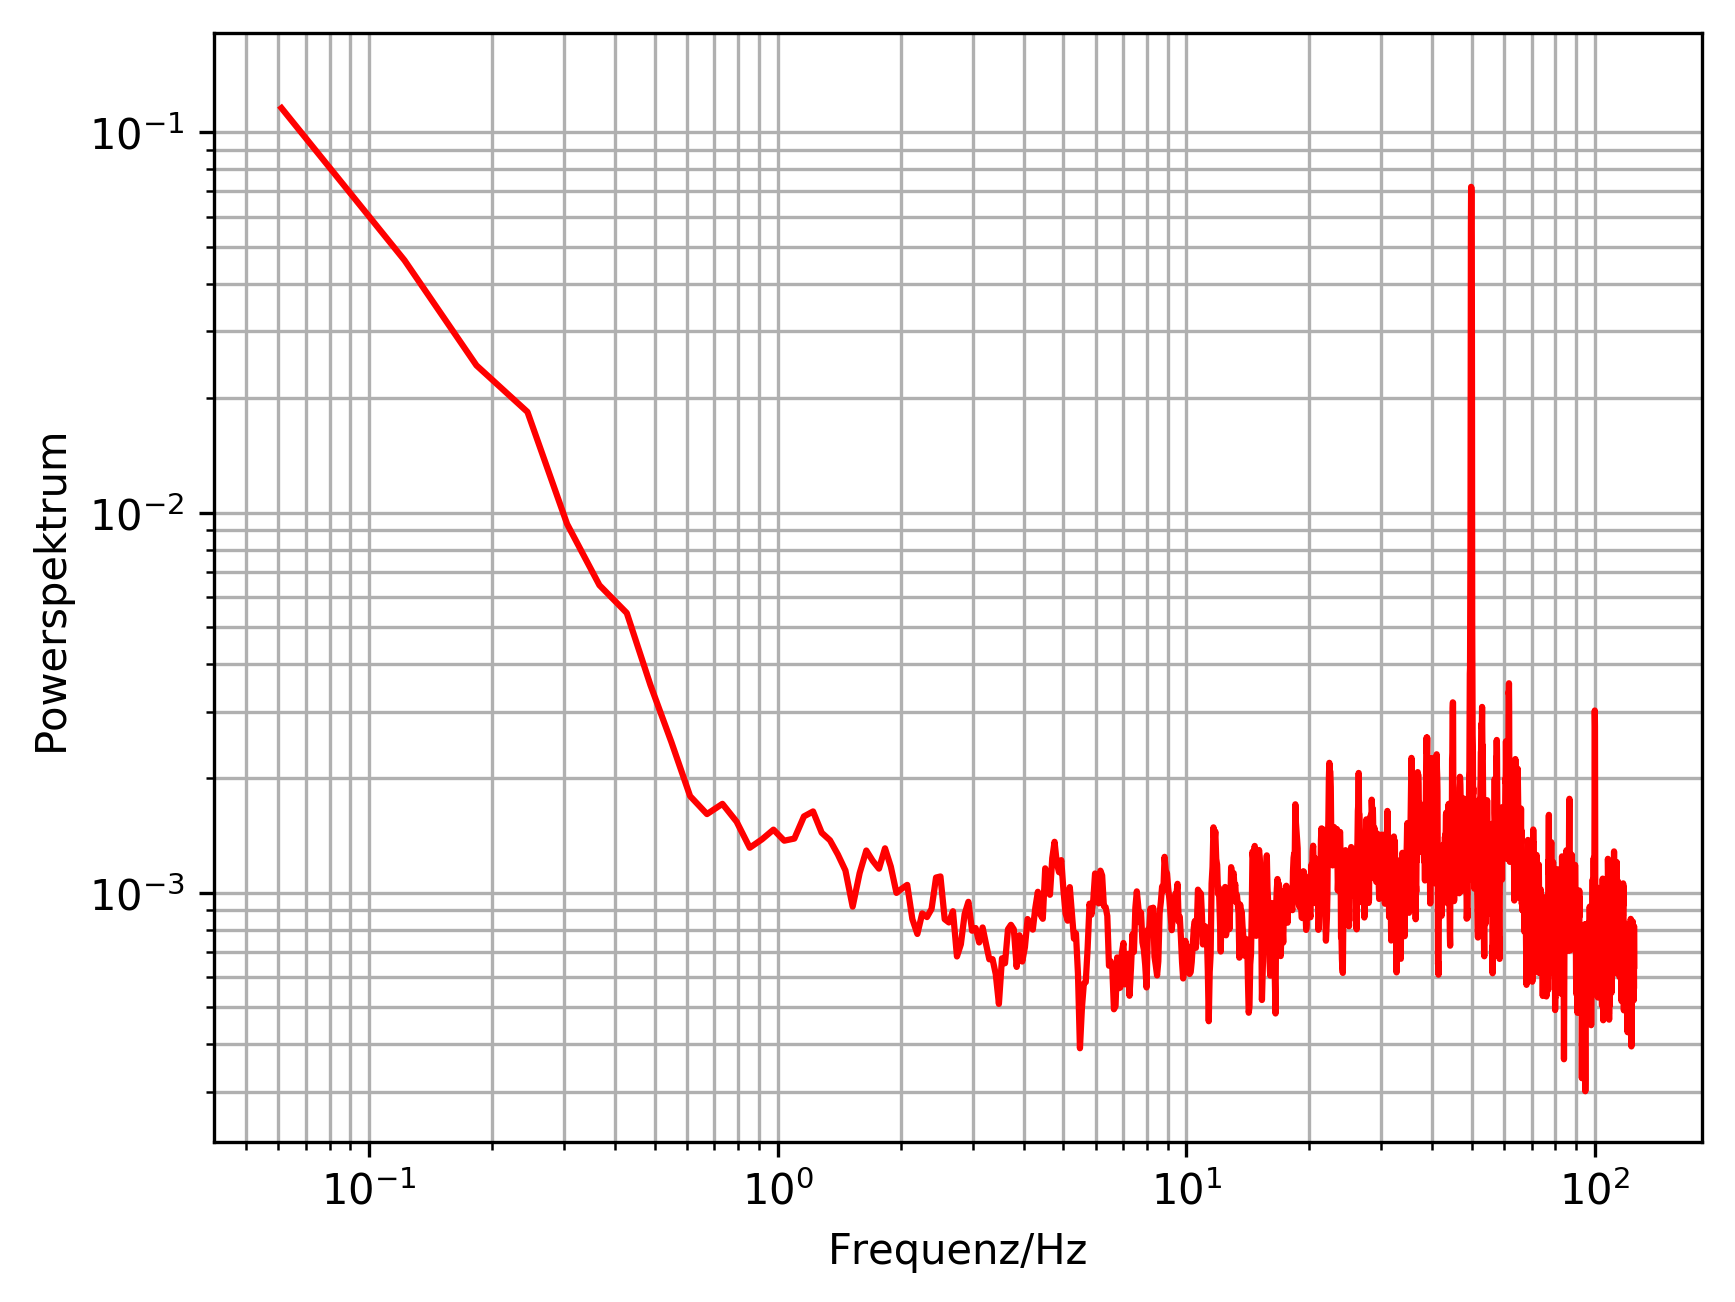
\includegraphics{stoer.png}
\caption{Störfrequenz Messung}
\label{fig:stoer}
\end{figure}



\subsection{Bestimmung der Abruchfrequenz}
%Michael fragen wegen der Formel



\subsection{Geschwindigkeits- und Temperaturprofil}
\label{sec:profile}

\begin{figure}[!ht]
\centering
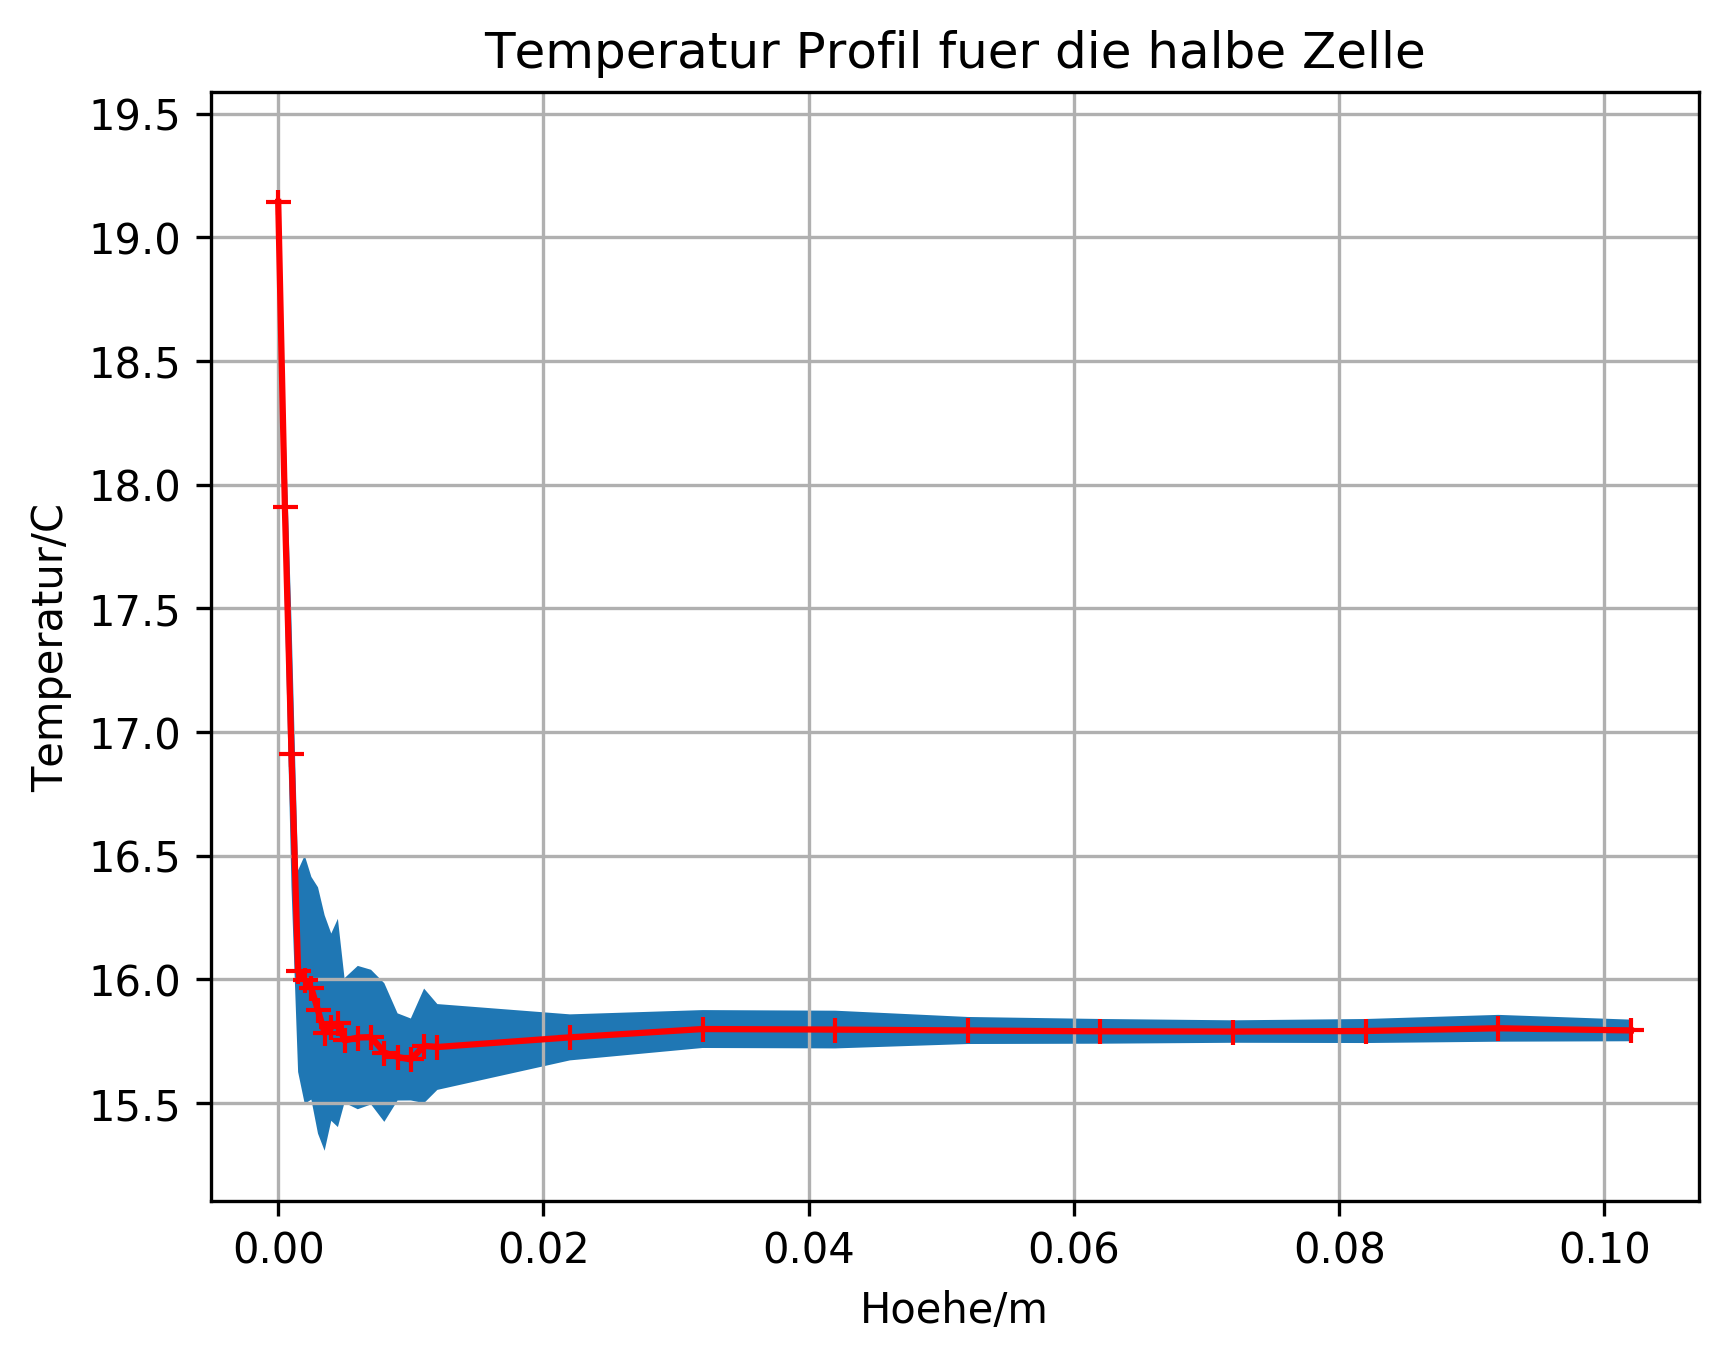
\includegraphics[width=0.8\textwidth]{T_fahrt.png}
\caption{Gemessenes Temperatur profil}
\label{fig:T_fahrt}
\end{figure}


\subsection{Numerische Profile und Daten}
\begin{figure}[!ht]
\centering
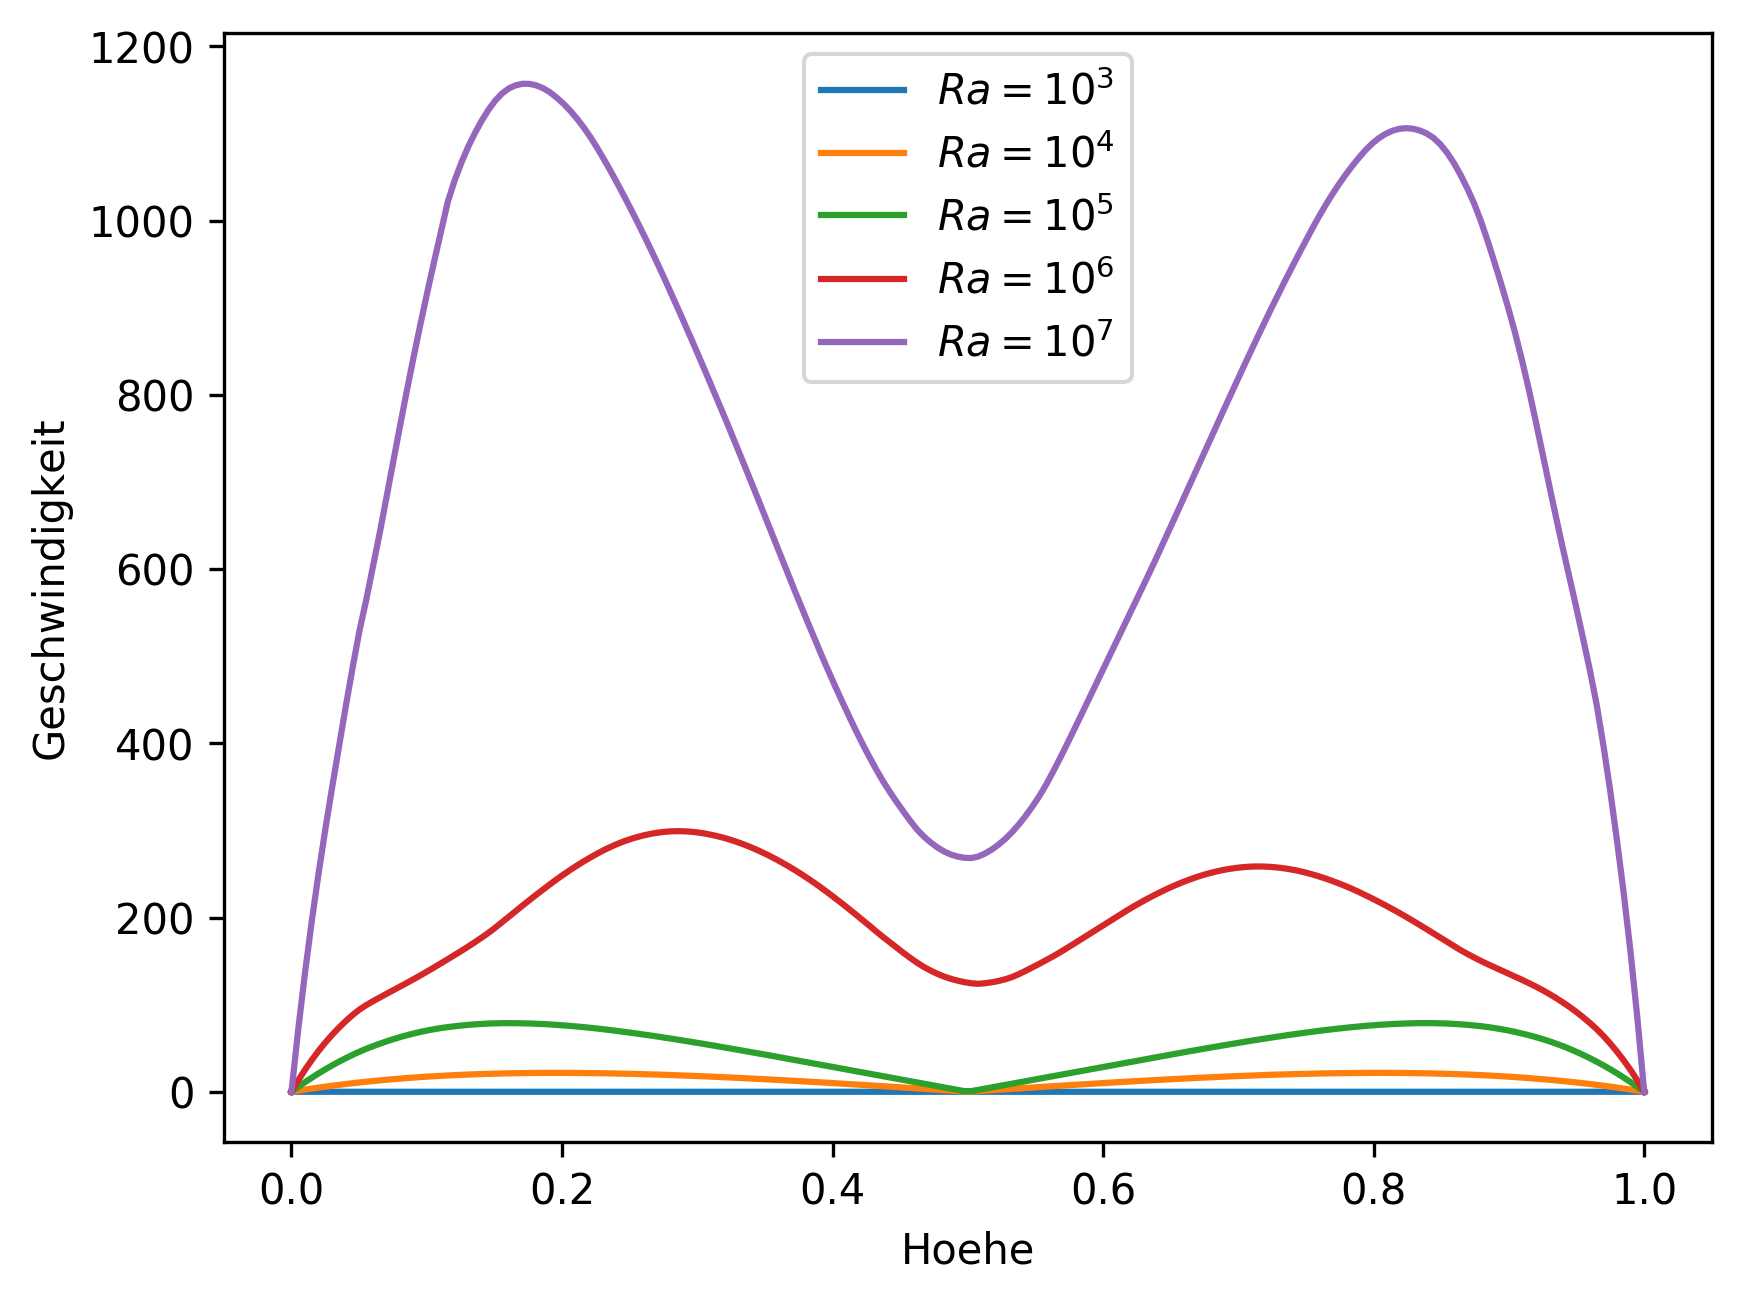
\includegraphics[width=0.8\textwidth]{V.png}
\caption{Geschwindigkeits profile}
\label{fig:v_num}
\end{figure}

\begin{figure}[!ht]
\centering
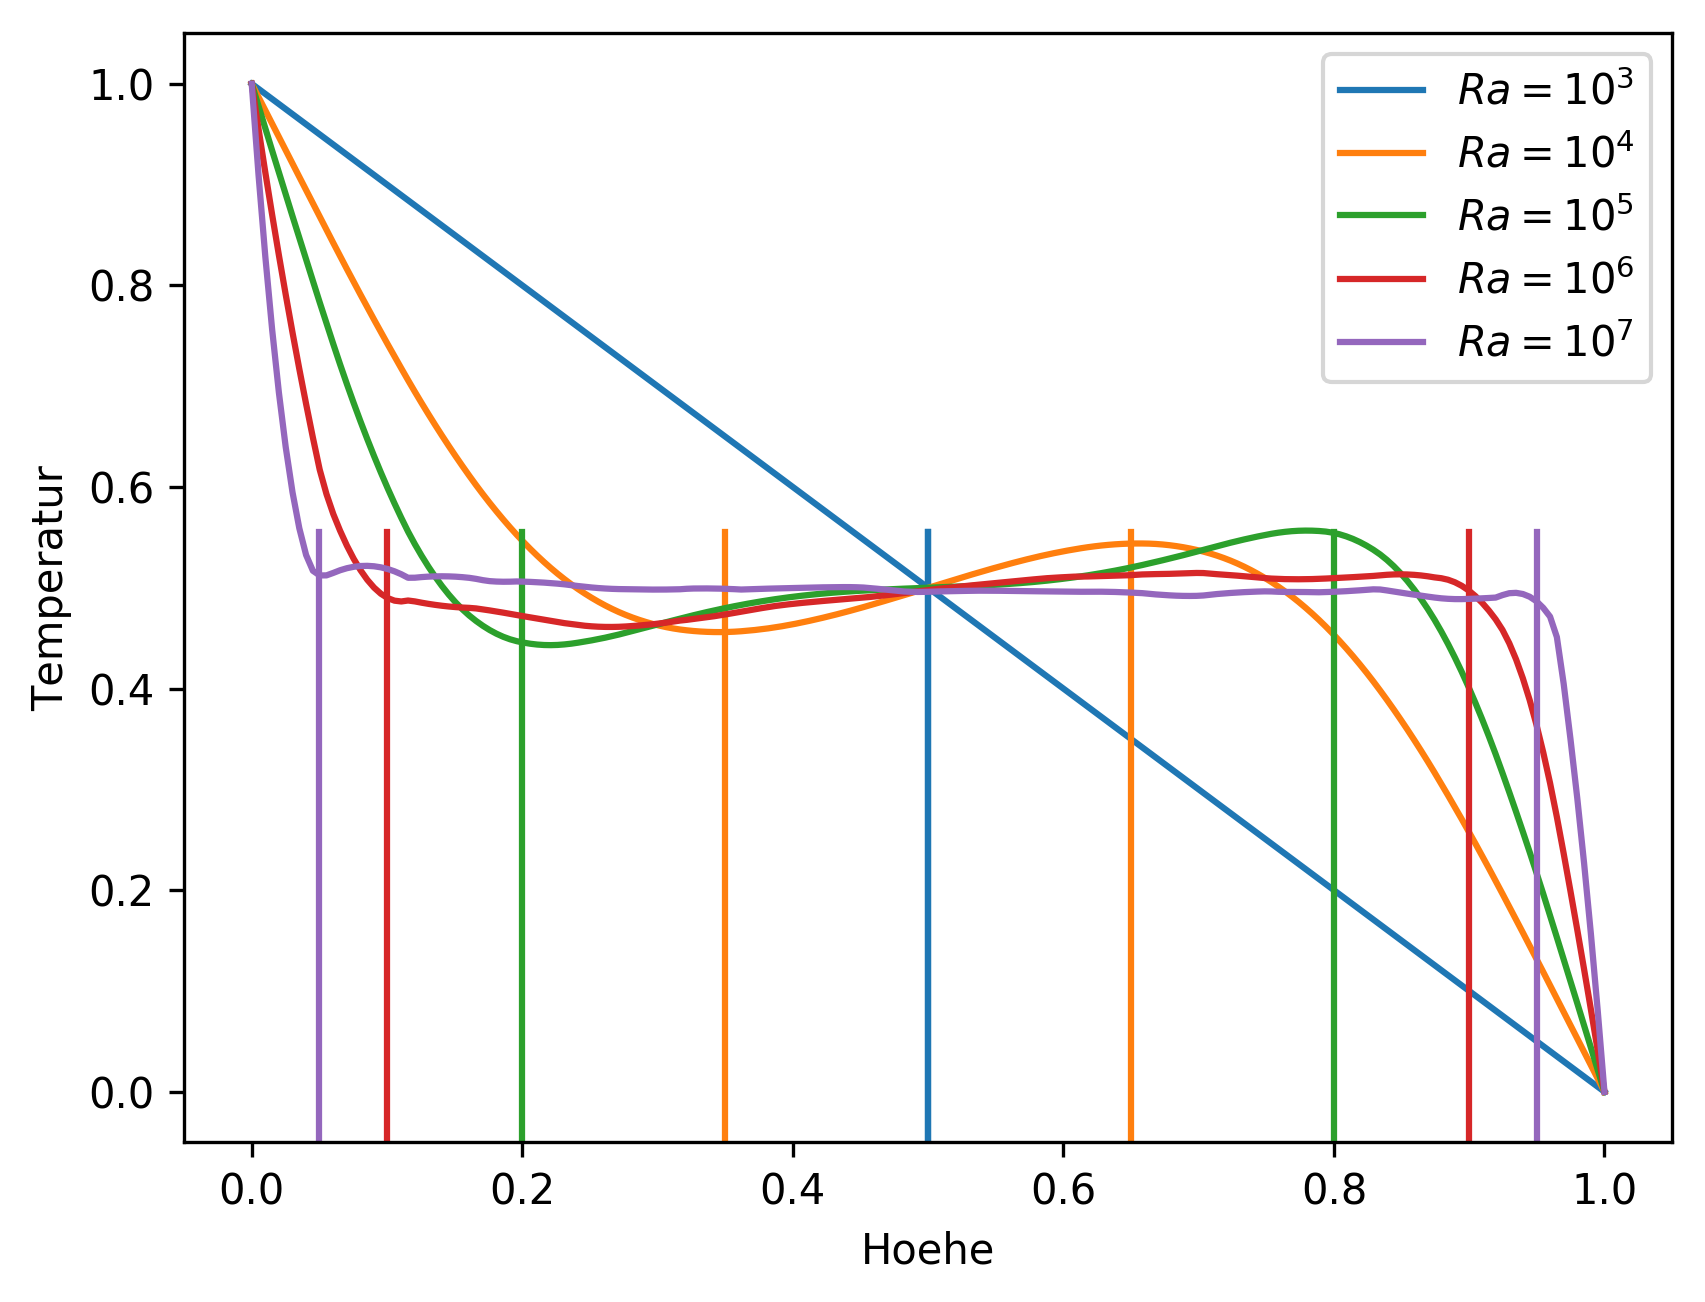
\includegraphics[width=0.8\textwidth]{T.png}
\caption{Temperatur profile}
\label{fig:t_num}
\end{figure}

\begin{figure}[!ht]
\centering
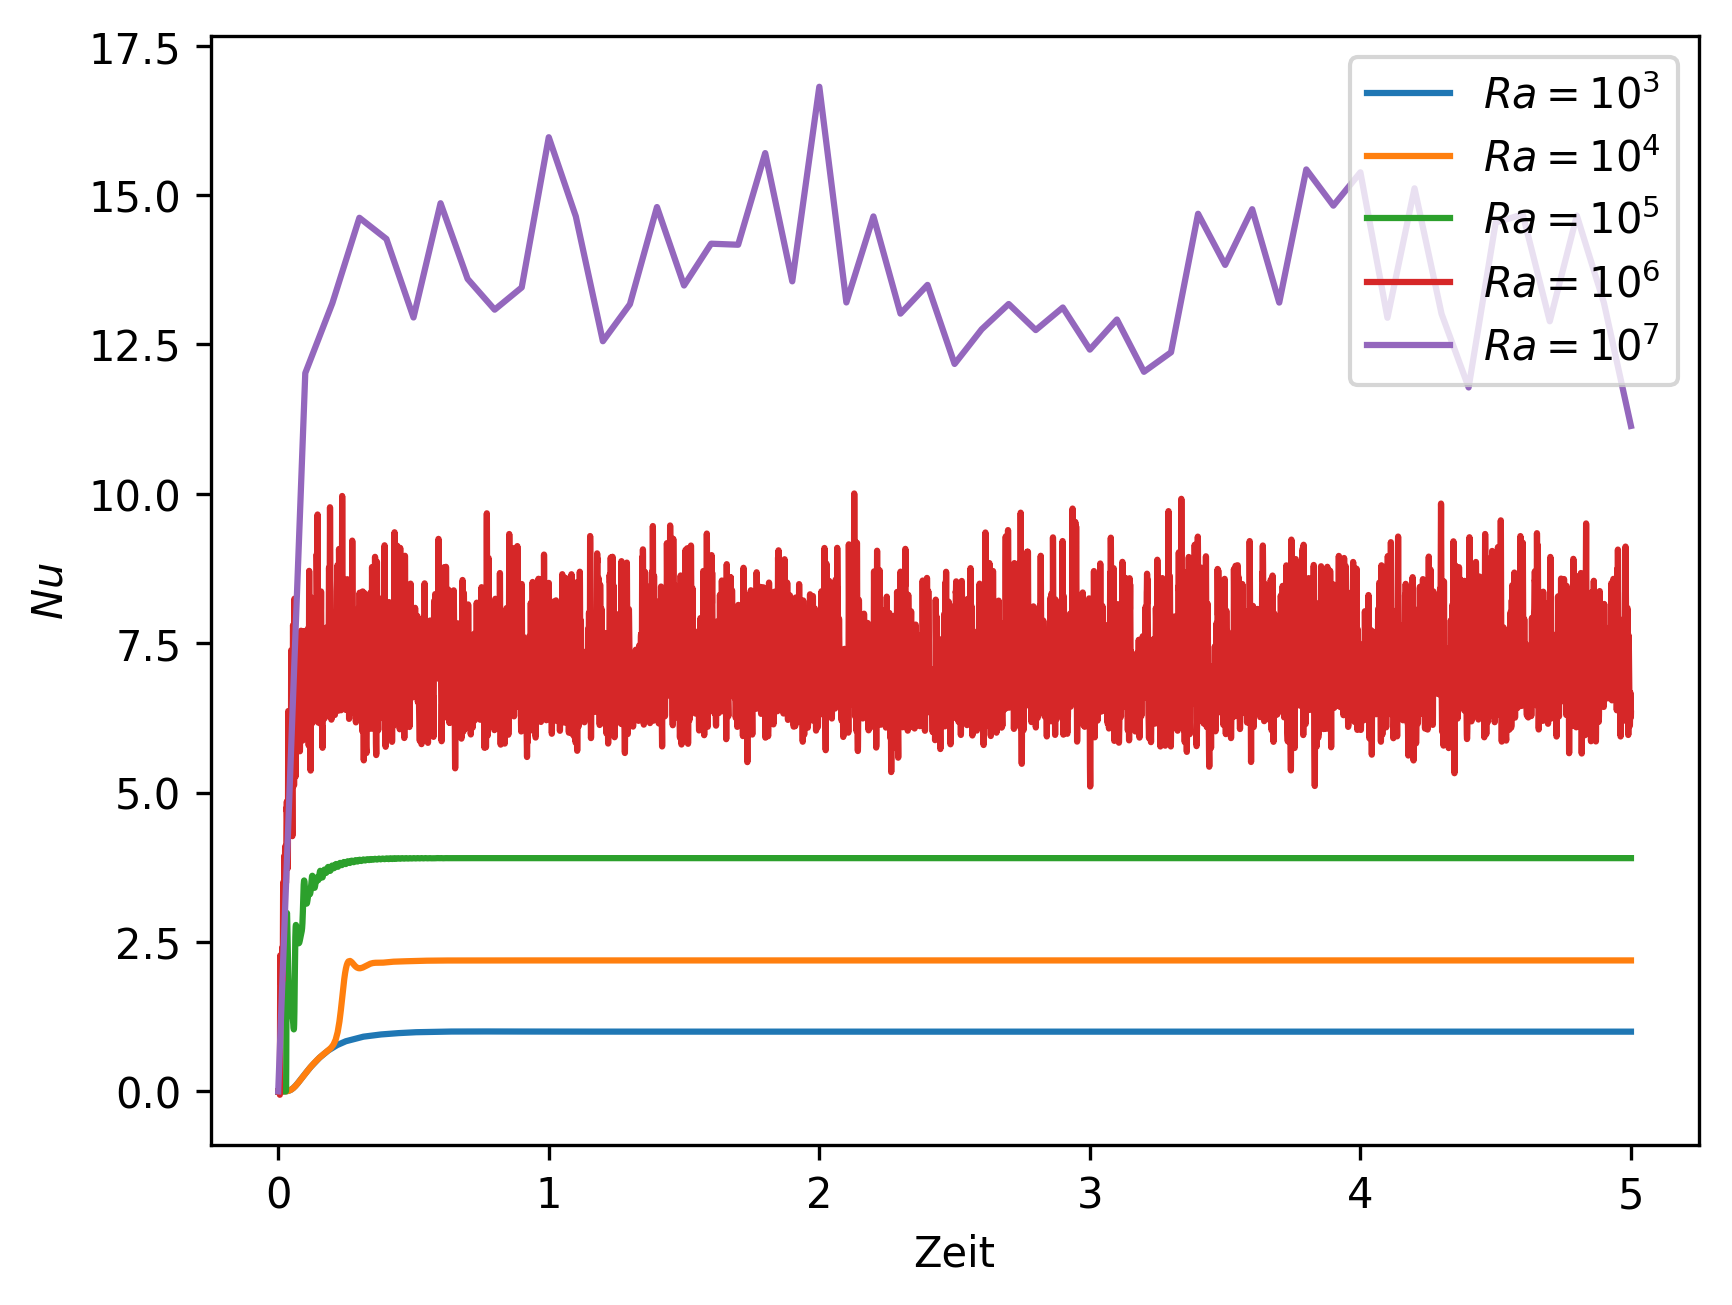
\includegraphics[width=0.8\textwidth]{Nu.png}
\caption{Nusselt Zahl}
\label{fig:nu_num}
\end{figure}





\subsection{Korellation}

\begin{figure}[!ht]
\centering
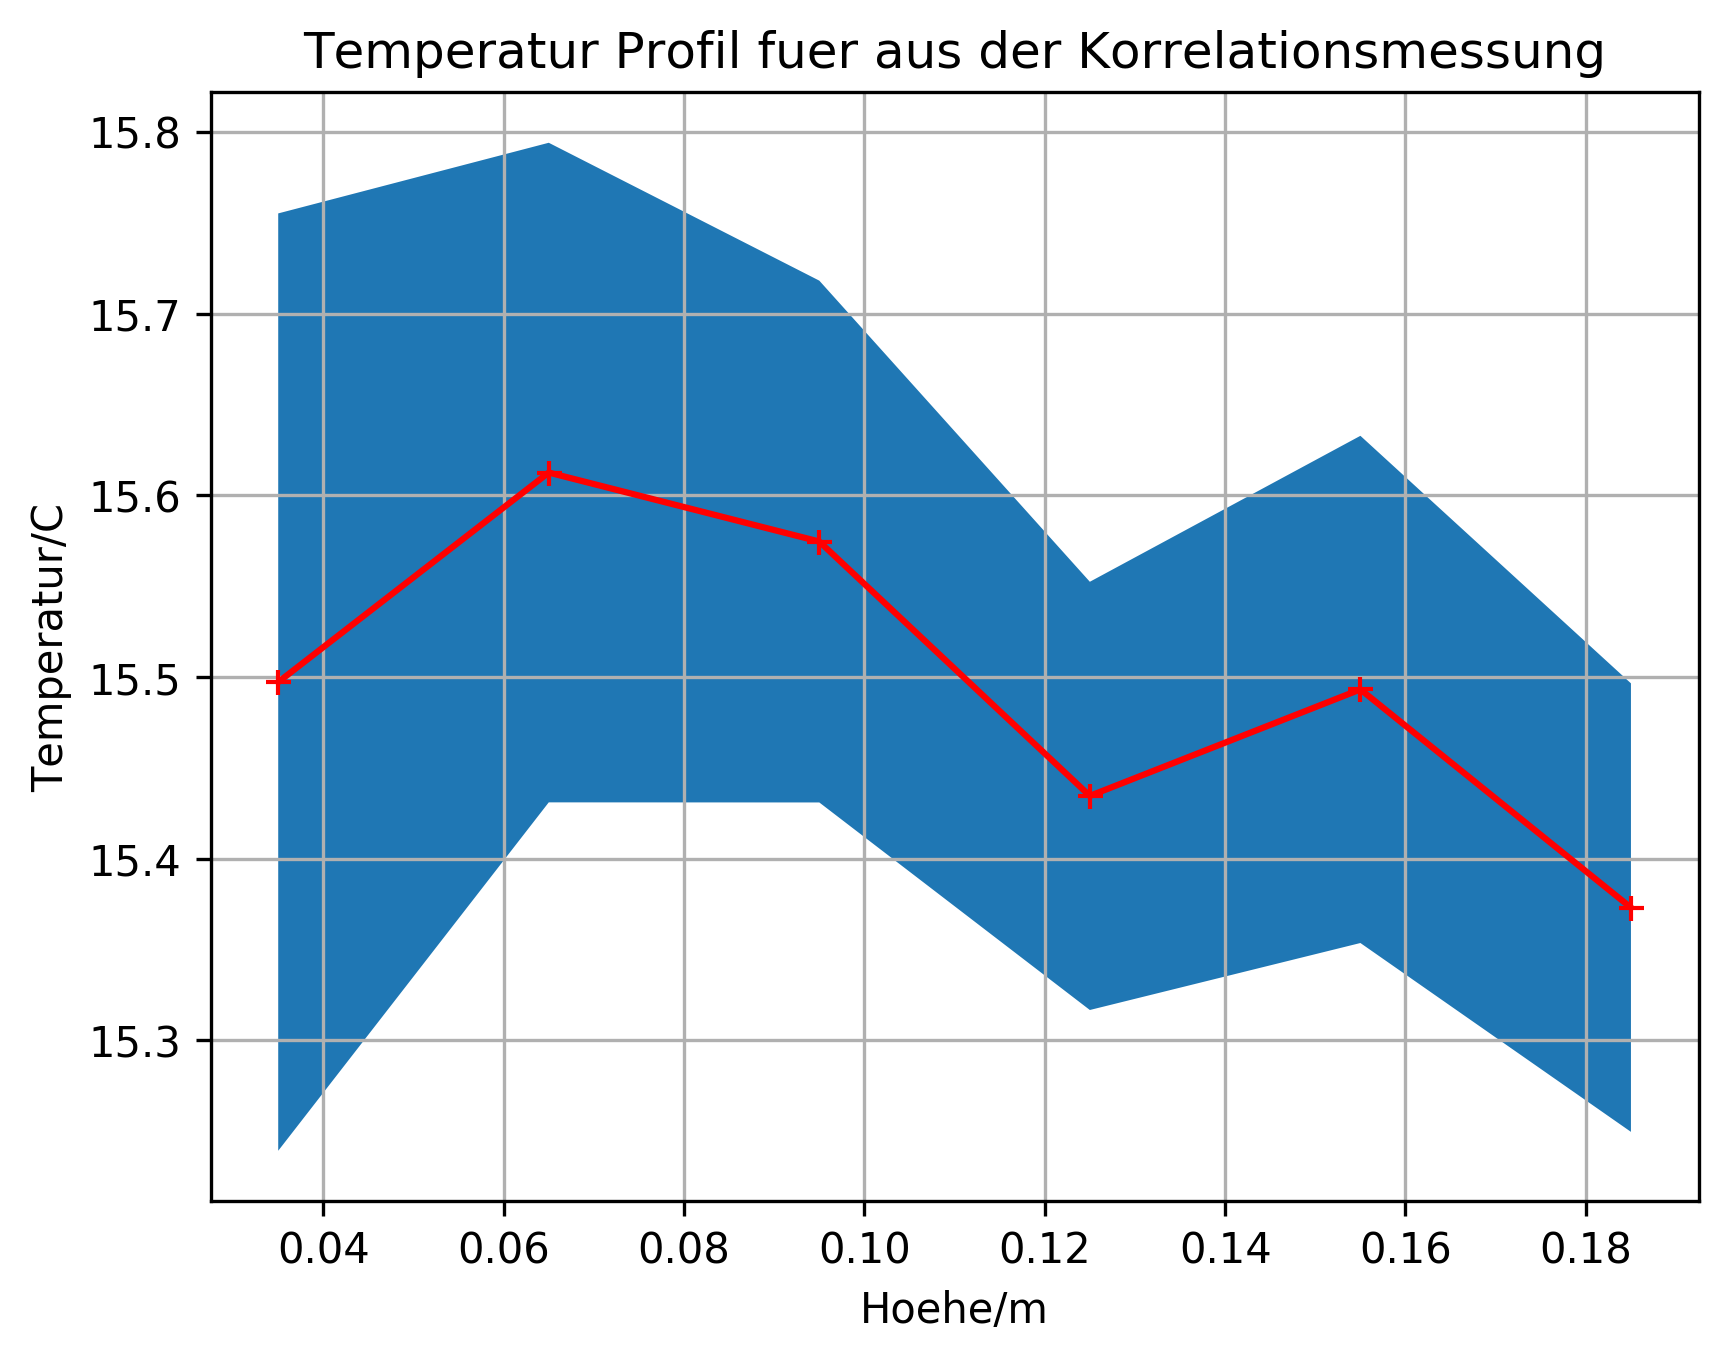
\includegraphics[width=0.8\textwidth]{T_kor.png}
\caption{Temperatur aus der Korrelatiionsmessung}
\label{fig:T_kor}
\end{figure}





\subsection{Vergleiche der Geschwindigkeiten}

\subsection{Nusselt-Zahl}

\begin{figure}[!ht]
\centering
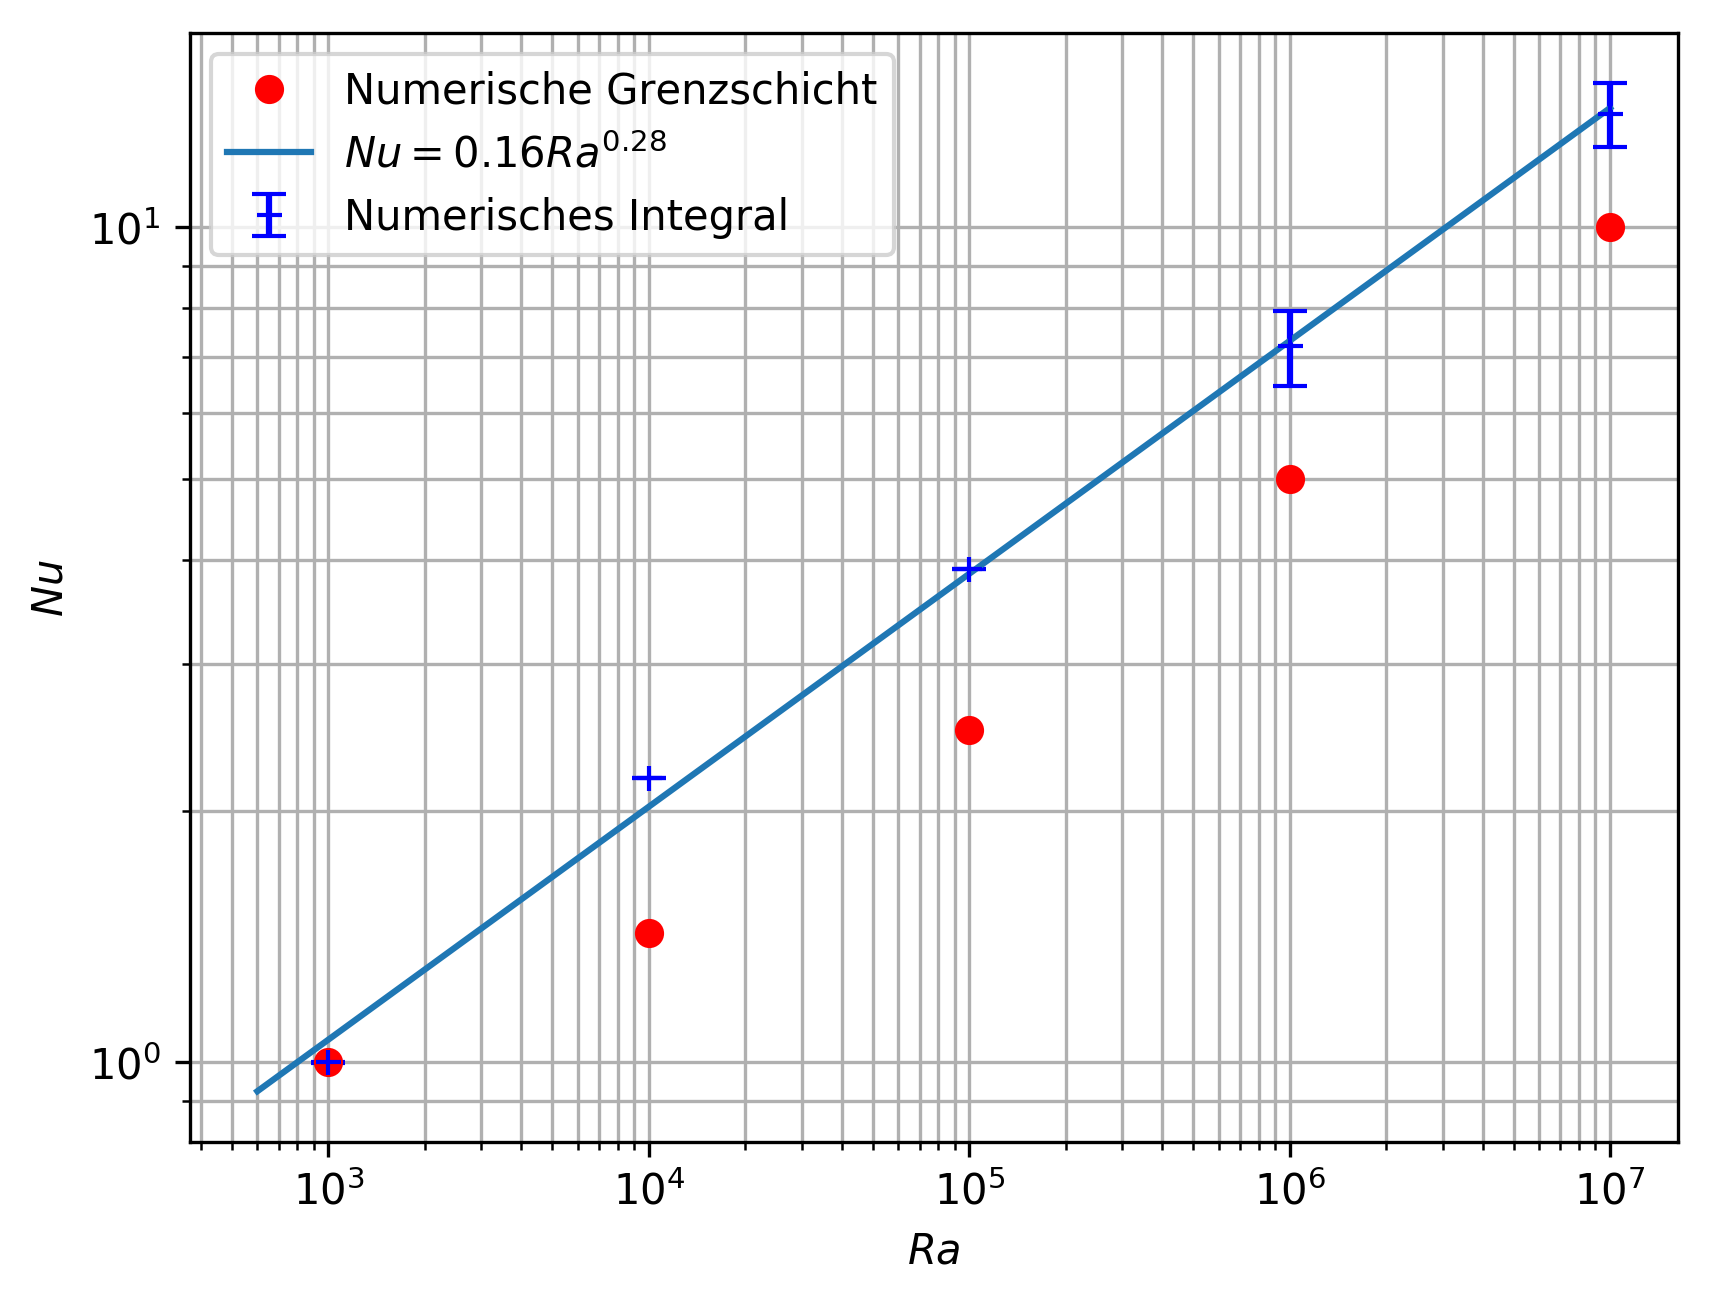
\includegraphics[width=0.8\textwidth]{Nu_Ra.png}
\caption{Nussel Zahl gegen Rayleigh Zahl aufgetragen.}
\label{fig:Nu_Ra}
\end{figure}






\subsection{Temperaturhistogramme}

\begin{figure}[!ht]
\centering
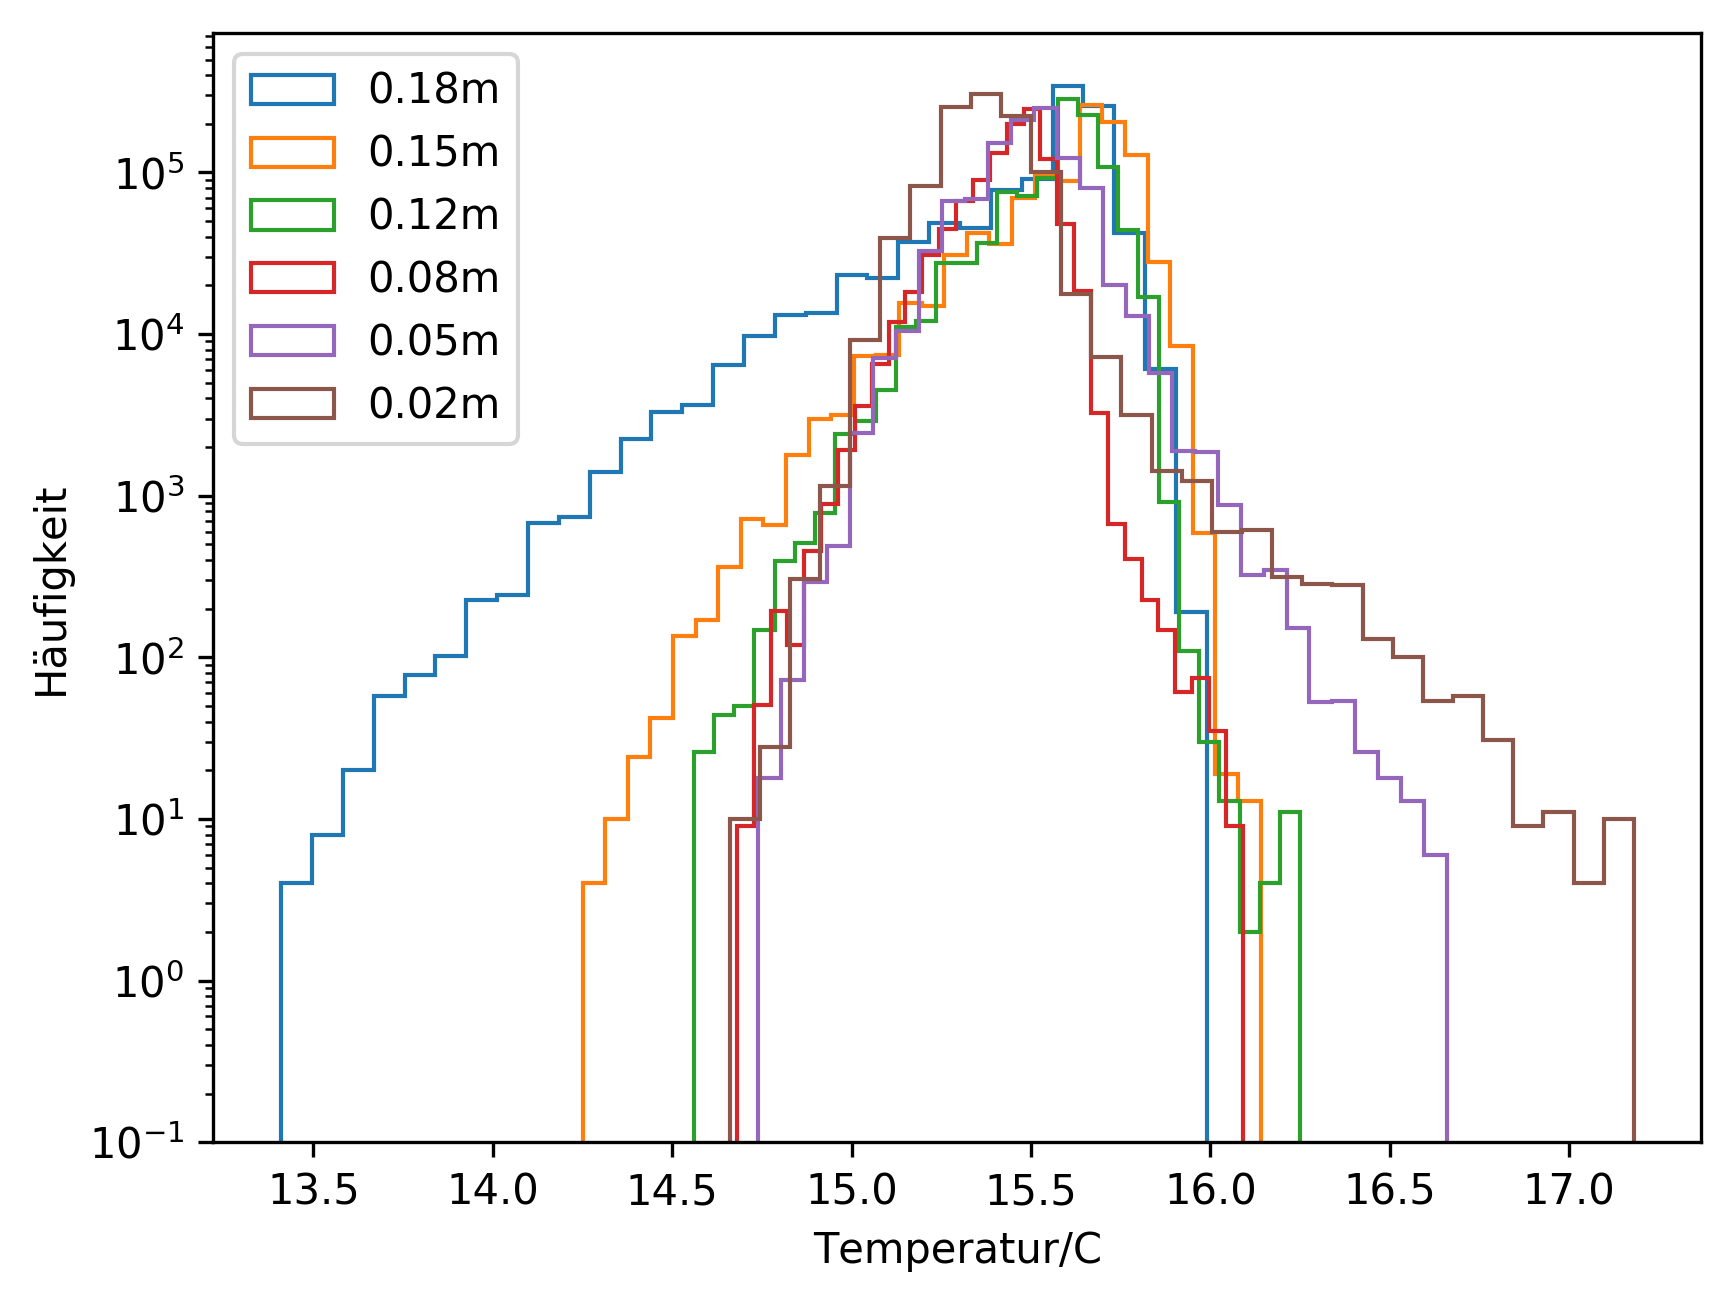
\includegraphics[width=0.8\textwidth]{hist.png}
\caption{Histogram der Temperaturen}
\label{fig:hist}
\end{figure}


\newpage
\section{Bewertung der Ergebnisse}
\label{sec:diskussion}

\newpage
\section{Anhang}
%Zahlen Überarbeiten und runden
\begin{table}
\centering
\begin{tabular}{|l|rrrr|}
\hline
                                            &          Zelle &         Erdkern &      Erdmantel &    Atmosph\"are \\
\hline\hline
$\alpha~[\si{\per\kelvin}]$                  &    0.00021     &     1.2e-05     &    1.5e-05     &     0.0037      \\
$\rho~[\si{\kilo\gram\per\cubic\meter}]$     & 1000           & 12000           & 5000           &     1.29        \\
 $c_p~[\si{\joule\per\kilo\gram\per\kelvin}]$ & 4187           &   800           & 1200           &  1000           \\
 $\lambda~[\si{\watt\per\meter\per\kelvin}]$   &    0.6         &    30           &   10           &     0.03        \\
 $\mu~[\si{\pascal\second}]$                  &    0.001       &     0.012       &    1e+21       &     1.7e-05     \\
 $\nu~[\si{\square\meter\per\second}]$        &    1e-06       &     1e-06       &    2e+17       &     1.31783e-05 \\
 $\kappa~[\si{\square\meter\per\second}]$     &    1.43301e-07 &     3.125e-06   &    1.66667e-06 &     2.32558e-05 \\
 $L~[\si{\meter}]$                            &    0.2         &     2.26e+06    &    2.855e+06   & 15000           \\
 $dT~[\si{\kelvin}]$                          &   10           &  2000           & 1000           &    65           \\
 $Pr$                                       &    6.97833     &     0.32        &    1.2e+23     &     0.566667    \\
 $Ra$                                       &    1.15009e+09 &     8.69672e+29 &    1.02731e+07 &     2.59817e+22 \\
\hline
\end{tabular}
\caption{Tabelle der Parameter und wichtige Stoffgrößen}
\label{tab:par}
\end{table}

\newpage
%\nocite{*} %sorgt dafuer, dass alles ausgegeben wird
\printbibliography[heading=bibintoc]
\end{document}
